%!TEX root = ../main.tex
% TODO considerazioni generali:
%[check] 1) togliere i riquadri: il lettore si riquadra quello che vuole e non servono a granché
%[check] 3) controllare che tutti i teoremi, definizioni, etc siano il più possibile completi e autosufficienti. Per esempio, se si parla di soluzione ai minimi quadrati, si dovrebbe anche scrivere qualcosa tipo "di un certo sistema lineare" o "del sistema lineare Ax=b". Mettere ref a equazioni troppo grosse per essere copiaincollate va benissimo però.
%[check] 4) Ci sono un po' di corsivi e grassetti abbastanza a caso o non necessari. Probabilmente Aron abolirà i grassetti, quindi inizia a pensare cosa vuoi davvero evidenziare (per es., non certo il nome di un teorema se lo enunci la riga dopo)
%[check] 5) Si dovrebbe unificare, o togliere, osservazioni e nota bene, a meno che non siano state classificate così per un motivo preciso (ma non mi sembra)
%[check] 6) In generale, vedi se alcuni teoremi o simili senza interpretazione ne hanno bisogno di una, per es. "questa disuguaglianza fornisce una stima dell'errore" (a meno che non sia già stato detto prima)
%[check] Indice analitico (aiuto)

% TODO forse rivedere lo stile degli algoritmi? Magari più spaziati dal resto del testo?

\chapter{Introduzione all'analisi numerica}
\label{chap:introduzione}

% \textit{[Lezione 1 (9-03-2020)]}

%Vedi slides in PDF. Introduzione al corso.

% \textit{[Lezione 2 (10-03-2020)]}

In questo testo si affronteranno i concetti fondamentali dell'analisi numerica.
Proponiamo questo capitolo introduttivo in modo da dare qualche motivazione sull'utilità della materia.
In generale, quando studiamo un problema fisico, dopo aver determinato una \textit{formula} della soluzione è anche fondamentale saper calcolare numericamente, o approssimare, questa soluzione per la specifica istanza del problema in questione.
Nei casi reali, molto spesso la soluzione esatta ci è sconosciuta e non possiamo ottenerla in forma chiusa: il compito dell'analisi numerica sarà allora quello di trovare la migliore approssimazione possibile.
Un altro caso di interesse è la \textit{simulazione} di un certo fenomeno, per sapere come una struttura reagisce ai carichi, o se un vaso sanguigno è a rischio rottura per la sua particolare conformazione. In tutti questi casi abbiamo una procedura sequenziale composta da diverse fasi:
\begin{enumerate}
	\index{problema!fisico}
	\item Un \textbf{problema fisico (PF)}: è il punto di partenza, in cui analizziamo una data situazione nel mondo reale.
	\index{problema!matematico}
	\item Un \textbf{problema matematico (PM)}: scegliamo un modello matematico che rappresenti il (PF), traducendo le informazioni su di esso in formule ed eventualmente operando le dovute ipotesi semplificative.
  Per esempio, se si è in una situazione in cui l'attrito ha valori trascurabili e non è quindi determinante per il problema in questione, esso può essere ignorato in modo da semplificare le formule.
	\index{problema!numerico}
	\item Un \textbf{problema numerico (PN)}: significa compiere un'ulteriore traduzione, dalle equazioni del (PM) a una serie di algoritmi e schemi numerici che permettano a un computer di risolvere il (PM).
  Ricordiamo infatti che un computer è uno strumento ``stupido'': esegue tutte e sole le istruzioni che gli vengono fornite, molto velocemente, ma non è in grado di comprendere il significato di concetti come ``integrale'' o ``serie infinita''.
  Un computer è in grado di eseguire solo le operazioni di base, e deve necessariamente approssimare i numeri secondo il suo metodo di rappresentazione, rendendo quindi impossibile utilizzare risultati numerici completamente esatti.
  Per esempio, è possibile che eseguendo la divisione $2/2$ e visualizzando il risultato si trovi $1.000000002$.
  Questi errori sono qualcosa di cui bisogna tenere conto nel progettare un algoritmo.
\end{enumerate}
Non scontato è chiedersi perché \textit{complicarsi} la vita così.
La ragione è che spesso quando si studiano situazioni reali e si vuole un livello di precisione molto alto, si presentano dati e sistemi di $n$ equazioni dove $n$ è un numero che può valere anche $10 000$ o $100 000$.
Procedere a mano non è quindi fattibile.

Inoltre, prendendo per esempio lo studio della resistenza delle pareti di un vaso sanguigno o del cuore, la modellistica numerica fornisce un'accuratezza \textit{ineguagliabile} da qualunque test clinico, senza essere invasiva per il paziente.

Procediamo quindi ad analizzare un primo esempio, per illustrare meglio queste affermazioni.

\section{Problema esempio}
Vogliamo determinare la configurazione di equilibrio di un filo elastico fissato agli estremi e soggetto ad una generica forza verticale di intensità variabile. Questo è il nostro (PF).

\subsection{Formulazione forte}
Descriveremo ora una prima formulazione del problema.
In particolare, fissato un asse cartesiano orizzontale avente $x \in [0,1]$ come coordinata, si indichi con $f(x)$ l'intensità di tale forza per unità di massa nel punto $x$.
Detta $u(x)$ la funzione che descrive lo spostamento verticale del filo in $x$ rispetto alla posizione di riposo $u=0$, dobbiamo trovare $u(x)$ tale che:
\begin{equation}\tag{PM}
	\begin{cases}
		-u''(x) =f(x) \\
		u(0) =0        \\
		u(1) =0
	\end{cases} \ \ \ \ x\in ( 0,1) .
	\label{eq:formulazione-forte}
\end{equation}

Questo è il nostro \eqref{eq:formulazione-forte}.
Non entriamo nel dettaglio delle ragioni della scelta di questo modello per questa situazione fisica, in quanto non sono oggetto di questo corso.

\begin{figure}[htpb]
	\centering


	\tikzset{every picture/.style={line width=0.75pt}} %set default line width to 0.75pt

	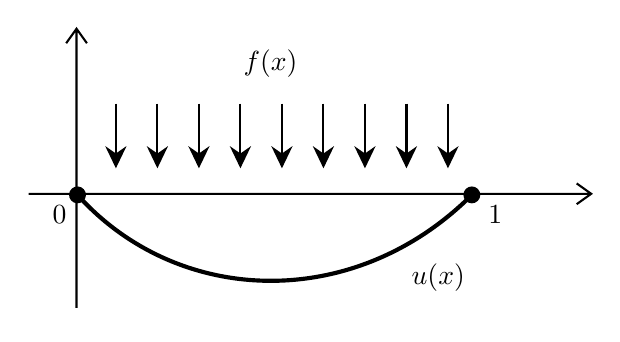
\begin{tikzpicture}[x=0.75pt,y=0.75pt,yscale=-1,xscale=1]
	%uncomment if require: \path (0,161); %set diagram left start at 0, and has height of 161

	%Shape: Axis 2D [id:dp2491153611335084]
	\draw  (123,93.29) -- (394,93.29)(146.04,13.75) -- (146.04,148.29) (387,88.29) -- (394,93.29) -- (387,98.29) (141.04,20.75) -- (146.04,13.75) -- (151.04,20.75)  ;
	%Curve Lines [id:da43974970723436657]
	\draw [line width=1.5]    (146.5,93.81) .. controls (195,147.75) and (280,150.25) .. (336.5,93.81) ;
	\draw [shift={(336.5,93.81)}, rotate = 315.03] [color={rgb, 255:red, 0; green, 0; blue, 0 }  ][fill={rgb, 255:red, 0; green, 0; blue, 0 }  ][line width=1.5]      (0, 0) circle [x radius= 3.05, y radius= 3.05]   ;
	\draw [shift={(146.5,93.81)}, rotate = 48.04] [color={rgb, 255:red, 0; green, 0; blue, 0 }  ][fill={rgb, 255:red, 0; green, 0; blue, 0 }  ][line width=1.5]      (0, 0) circle [x radius= 3.05, y radius= 3.05]   ;
	%Straight Lines [id:da9787839476649458]
	\draw    (165,49.81) -- (165,78) ;
	\draw [shift={(165,81)}, rotate = 270] [fill={rgb, 255:red, 0; green, 0; blue, 0 }  ][line width=0.08]  [draw opacity=0] (10.72,-5.15) -- (0,0) -- (10.72,5.15) -- (7.12,0) -- cycle    ;
	%Straight Lines [id:da9827078453458891]
	\draw    (185,49.81) -- (185,78) ;
	\draw [shift={(185,81)}, rotate = 270] [fill={rgb, 255:red, 0; green, 0; blue, 0 }  ][line width=0.08]  [draw opacity=0] (10.72,-5.15) -- (0,0) -- (10.72,5.15) -- (7.12,0) -- cycle    ;
	%Straight Lines [id:da17537912199596928]
	\draw    (205,49.81) -- (205,78) ;
	\draw [shift={(205,81)}, rotate = 270] [fill={rgb, 255:red, 0; green, 0; blue, 0 }  ][line width=0.08]  [draw opacity=0] (10.72,-5.15) -- (0,0) -- (10.72,5.15) -- (7.12,0) -- cycle    ;
	%Straight Lines [id:da49005928477817595]
	\draw    (225,49.81) -- (225,78) ;
	\draw [shift={(225,81)}, rotate = 270] [fill={rgb, 255:red, 0; green, 0; blue, 0 }  ][line width=0.08]  [draw opacity=0] (10.72,-5.15) -- (0,0) -- (10.72,5.15) -- (7.12,0) -- cycle    ;
	%Straight Lines [id:da8291729805680772]
	\draw    (245,49.81) -- (245,78) ;
	\draw [shift={(245,81)}, rotate = 270] [fill={rgb, 255:red, 0; green, 0; blue, 0 }  ][line width=0.08]  [draw opacity=0] (10.72,-5.15) -- (0,0) -- (10.72,5.15) -- (7.12,0) -- cycle    ;
	%Straight Lines [id:da329222982718808]
	\draw    (265,49.81) -- (265,78) ;
	\draw [shift={(265,81)}, rotate = 270] [fill={rgb, 255:red, 0; green, 0; blue, 0 }  ][line width=0.08]  [draw opacity=0] (10.72,-5.15) -- (0,0) -- (10.72,5.15) -- (7.12,0) -- cycle    ;
	%Straight Lines [id:da08987398027034099]
	\draw    (285,49.81) -- (285,78) ;
	\draw [shift={(285,81)}, rotate = 270] [fill={rgb, 255:red, 0; green, 0; blue, 0 }  ][line width=0.08]  [draw opacity=0] (10.72,-5.15) -- (0,0) -- (10.72,5.15) -- (7.12,0) -- cycle    ;
	%Straight Lines [id:da6194516261208358]
	\draw    (305,49.81) -- (305,78) ;
	\draw [shift={(305,81)}, rotate = 270] [fill={rgb, 255:red, 0; green, 0; blue, 0 }  ][line width=0.08]  [draw opacity=0] (10.72,-5.15) -- (0,0) -- (10.72,5.15) -- (7.12,0) -- cycle    ;
	%Straight Lines [id:da9977004284286]
	\draw    (325,49.81) -- (325,78) ;
	\draw [shift={(325,81)}, rotate = 270] [fill={rgb, 255:red, 0; green, 0; blue, 0 }  ][line width=0.08]  [draw opacity=0] (10.72,-5.15) -- (0,0) -- (10.72,5.15) -- (7.12,0) -- cycle    ;

	% Text Node
	\draw (133,97.4) node [anchor=north west][inner sep=0.75pt]    {$0$};
	% Text Node
	\draw (343,97.4) node [anchor=north west][inner sep=0.75pt]    {$1$};
	% Text Node
	\draw (306,125.4) node [anchor=north west][inner sep=0.75pt]    {$u(x)$};
	% Text Node
	\draw (225,22.4) node [anchor=north west][inner sep=0.75pt]    {$f(x)$};


	\end{tikzpicture}
\end{figure}
\FloatBarrier

Per ogni $f\in C^{0}([ 0,1])$ esiste un'unica soluzione $u\in C^{2}([ 0,1])$ del problema \eqref{eq:formulazione-forte} che ammette la seguente rappresentazione:
\begin{equation}
	u(x) =x\int ^{1}_{0}( 1-s) f(s) ds-\int ^{x}_{0}( x-s) f(s) \ds.
\label{eq:formulazione-forte-soluzione}
\end{equation}
\textit{Dimostrazione.}

Separiamo le variabili e integriamo
\begin{equation*}
-\frac{du'( x)}{\dx} =f( x) \ \ \Rightarrow \ \ -du'( x) =f( x) \dx\ \ \Rightarrow \ \ -\int ^{x}_{0} du'( s) =\int ^{x}_{0} f( s) \ds.
\end{equation*}
Il risultato dell'integrazione è
\begin{equation*}
u'( x) -u'( 0) =-\int ^{x}_{0} f( s) \ds\ \ \Rightarrow \ \ u'( x) =-\int ^{x}_{0} f( s) \ds+c_{1},
\end{equation*}
integrando quindi ulteriormente con la stessa procedura
\begin{equation*}
u( x) =-\int ^{x}_{0} F( s) \ds+c_{1} x+c_{2} ,\ \ \text{indicando} \ F( s) =\int ^{s}_{0} f( t) \dt.
\end{equation*}
Integrando per parti il termine $\int ^{x}_{0} F( s) \ds$:
\begin{align*}
\int ^{x}_{0} F( s) \ds & \overset{\text{ipp}}{=}[ sF( s)]^{x}_{0} -\int ^{x}_{0} sF'( s) \ds\\
 & =\left[ xF( x) -\cancel{0F( 0)}\right] -\int ^{x}_{0} sf( s) \ds\\
 & =x\int ^{x}_{0} f( s) \ds-\int ^{x}_{0} sf( s) \ds\\
 & =\int ^{x}_{0} f( s)( x-s) \ds,
\end{align*}
da cui
\begin{equation*}
u( x) =-\int ^{x}_{0} f( s)( x-s) \ds+c_{1} x+c_{2}.
\end{equation*}
Le costanti $c_{1} ,c_{2}$ le otteniamo imponendo le condizioni al bordo $u( 0) =u( 1) =0$:
\begin{align*}
0=u( 0) & =\cancel{-\int ^{0}_{0} f( s)( 0-s) \ds} +\cancel{c_{1} \cdot 0} +c_{2} =c_{2}\\
 & \Rightarrow \ \ c_{2} =0\\
0=u( 1) & =-\int ^{1}_{0} f( s)( 1-s) \ds+c_{1} \cdot 1+\cancel{c_{2}}\\
 & \Rightarrow \ \ c_{1} =\int ^{1}_{0} f( s)( 1-s) \ds.
\end{align*}
Sostituendo, otteniamo la \eqref{eq:formulazione-forte-soluzione}.\textqed
%TODO ARON qui aggiungere un accapo/spazio?
% Con il doppio accapo c'è già uno spazio, e io personalmente non sono molto un
% fan dello spazio extra "per delimitare".
% Se comunque ne vuoi possiamo metterne un po'. (AW)

Si può dimostrare inoltre che se $f\in C^{m}([ 0,1])$, $m\geqslant 0$, allora $u\in C^{m+2}([ 0,1])$.

La $f(x)$ è detta \textit{forzante} e rappresenta l'azione esogena, proveniente dall'esterno del sistema di cui studiamo l'evoluzione. Cosa succede se $f\notin C^{0}([ 0,1])$, cioè se vogliamo studiare stimoli discontinui a tratti? È chiaro che se alla corda agganciamo una massa nel suo punto medio allora assumerà una configurazione a triangolo:
\begin{figure}[htpb]
	\centering
	\tikzset{every picture/.style={line width=0.75pt}} %set default line width to 0.75pt

	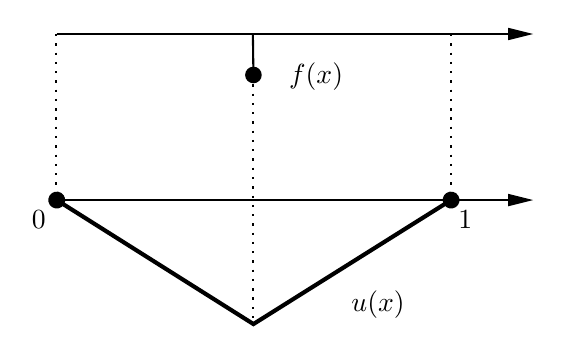
\begin{tikzpicture}[x=0.75pt,y=0.75pt,yscale=-1,xscale=1]
	%uncomment if require: \path (0,285); %set diagram left start at 0, and has height of 285

	%Straight Lines [id:da7930734499899124]
	\draw [line width=1.5]    (150.5,140) -- (245.27,199.74) -- (340.5,140) ;
	\draw [shift={(340.5,140)}, rotate = 327.9] [color={rgb, 255:red, 0; green, 0; blue, 0 }  ][fill={rgb, 255:red, 0; green, 0; blue, 0 }  ][line width=1.5]      (0, 0) circle [x radius= 3.05, y radius= 3.05]   ;
	\draw [shift={(150.5,140)}, rotate = 32.23] [color={rgb, 255:red, 0; green, 0; blue, 0 }  ][fill={rgb, 255:red, 0; green, 0; blue, 0 }  ][line width=1.5]      (0, 0) circle [x radius= 3.05, y radius= 3.05]   ;
	%Straight Lines [id:da8735021769677791]
	\draw    (150.5,140) -- (378,140) ;
	\draw [shift={(380,140)}, rotate = 180] [fill={rgb, 255:red, 0; green, 0; blue, 0 }  ][line width=0.08]  [draw opacity=0] (12,-3) -- (0,0) -- (12,3) -- cycle    ;
	%Straight Lines [id:da15555188364411165]
	\draw    (150.5,60) -- (378,60) ;
	\draw [shift={(380,60)}, rotate = 180] [fill={rgb, 255:red, 0; green, 0; blue, 0 }  ][line width=0.08]  [draw opacity=0] (12,-3) -- (0,0) -- (12,3) -- cycle    ;
	%Shape: Circle [id:dp8335871351332671]
	\draw  [draw opacity=0][fill={rgb, 255:red, 0; green, 0; blue, 0 }  ,fill opacity=1 ] (241.27,79.74) .. controls (241.27,77.53) and (243.06,75.74) .. (245.27,75.74) .. controls (247.48,75.74) and (249.27,77.53) .. (249.27,79.74) .. controls (249.27,81.95) and (247.48,83.74) .. (245.27,83.74) .. controls (243.06,83.74) and (241.27,81.95) .. (241.27,79.74) -- cycle ;
	%Straight Lines [id:da9075165176159563]
	\draw  [dash pattern={on 0.84pt off 2.51pt}]  (150,60) -- (150,140) ;
	%Straight Lines [id:da9403890066543903]
	\draw  [dash pattern={on 0.84pt off 2.51pt}]  (245.27,79.74) -- (245.27,199.74) ;
	%Straight Lines [id:da4334060500160668]
	\draw  [dash pattern={on 0.84pt off 2.51pt}]  (340.5,60) -- (340.5,140) ;
	%Straight Lines [id:da28452470752063985]
	\draw    (245.27,79.74) -- (245,60) ;

	% Text Node
	\draw (137,143.59) node [anchor=north west][inner sep=0.75pt]    {$0$};
	% Text Node
	\draw (342.5,143.4) node [anchor=north west][inner sep=0.75pt]    {$1$};
	% Text Node
	\draw (291,182.4) node [anchor=north west][inner sep=0.75pt]    {$u( x)$};
	% Text Node
	\draw (261,72.4) node [anchor=north west][inner sep=0.75pt]    {$f( x)$};
	\end{tikzpicture}
\end{figure}
\FloatBarrier
Anche considerare forzanti continue a tratti è di grande interesse fisico.
Tuttavia, queste non possono essere trattate con la formulazione \eqref{eq:formulazione-forte}, che è detta \textbf{formulazione forte}\index{formulazione!forte}, in quanto essa è troppo limitata a scelte di $f$ regolare.
Ci proponiamo quindi di espandere il concetto di soluzione con la seguente nuova formulazione.
\subsection{Formulazione debole}
\label{sec:formulazione-debole}

Vogliamo passare da un problema differenziale del secondo ordine ad uno in forma integrale del primo ordine (\textbf{formulazione debole})\index{formulazione!debole}\footnote{I seguenti passaggi potrebbero risultare un po' nebulosi.
Ciò non deve scoraggiare perché è solo per dare qualche motivazione ai vari argomenti che si affronteranno nel corso. Inoltre, gran parte di questi contenuti più teorici (funzioni test, spazi $L^{p}$, spazi a dimensione infinita) verranno approfonditi in corsi successivi.}.

Formalmente moltiplichiamo l'equazione \eqref{eq:formulazione-forte} per una funzione $v\in V$, detta \textit{funzione test}, ed integriamo tra $0$ e $1$:
\begin{equation*}
	-u''(x) =f(x)\ \ \Rightarrow\ \ \int\nolimits ^{1}_{0} -u''(x) v(x) \dx=\int\nolimits ^{1}_{0} f(x) v(x) \dx.
\end{equation*}
Per il momento supponiamo che le operazioni siano tutte lecite; ci occuperemo dei dettagli formali, come la definizione dello spazio $V$, in un secondo momento.
Integriamo il primo integrale per parti, con lo scopo di far scomparire la derivata seconda di $u$:
\begin{equation*}
	\int\nolimits ^{1}_{0} u'(x) v'(x) \dx-[ u'(x) v(x)]^{1}_{0} =\int\nolimits ^{1}_{0} f(x) v(x) \dx.
\end{equation*}
Si può dimostrare\footnote{ma non è argomento di questo testo.} che poiché la soluzione è fissa agli estremi $u(0) =u(1) =0$, allora la scelta ottimale delle funzioni test in $V$ è tale per cui esse siano nulle agli estremi dell'intervallo, cioè:
\begin{gather*}
	v\in V\ \ \Rightarrow \ \ v(0) =v(1) =0,\\
	\int\nolimits ^{1}_{0} u'(x) v'(x) \dx-\cancel{u'(1) v(1)} +\cancel{u'(0) v(0)} =\int\nolimits ^{1}_{0} f(x) v(x) \dx.
\end{gather*}
Definiamo lo spazio
\begin{equation*}
	L^{2}( 0,1) \coloneqq \left\{v:( 0,1)\rightarrow \mathbb{R} \ \text{tali che} \ \left(\int ^{1}_{0}| v| ^{2} \dx\right)^{1/2} < +\infty \right\} ,
\end{equation*}
e definiamo di conseguenza lo spazio $V$ come
\begin{equation*}
	V=\left\{v:( 0,1)\rightarrow \mathbb{R} \ |\ v\in L^{2}( 0,1) ,\ v'\in L^{2}( 0,1) ,\ v(0) =v(1) =0\right\} .
\end{equation*}
Arriviamo così alla formulazione debole del problema. Data $f \in L^{2}(0,1)$ trovare $u \in V$ tale che:
\begin{equation}\tag{PM'}
	\displaystyle\int\nolimits ^{1}_{0} u'(x) v'(x) \dx=\int\nolimits ^{1}_{0} f(x) v(x) \dx,\ \ \ \ \forall v(x) \in V.
	\label{eq:formulazione-debole}
\end{equation}
\textit{La formulazione debole è quindi più generale di quella forte}, dal momento che non richiede che $f$ sia derivabile, ma formula la soluzione sotto forma di integrale. Di conseguenza la richiesta su $f$ sarà di integrabilità: lo spazio $L^{2} $ è infatti lo spazio di funzioni il cui quadrato è integrabile\footnote{Tra tutti gli spazi $L^{p} $ c'è una preferenza a scegliere $L^2$ dato che è l'unico ad essere uno spazio di Hilbert, e questo porta con sé una serie di interessanti e utili proprietà, non oggetto di questo corso.}.

\textit{Osservazioni.} % TODO GRAF vanno formattate meglio
\begin{itemize}
	\item In \eqref{eq:formulazione-debole} compare solo la derivata prima di $u$.
	\item Lo spazio $\displaystyle V$ è più grande dello spazio $\displaystyle C^{2}([ 0,1])$.
\end{itemize}
\subsection{Problema numerico}

Il prossimo obiettivo è costruire una successione approssimante $u_{h}$ della soluzione originale $u$ di \eqref{eq:formulazione-forte}, dove $u_{h}$ è soluzione di un problema \textit{simile} a \eqref{eq:formulazione-forte}, ma che sia finito-dimensionale, al contrario del problema ``originale'' che è infinito-dimensionale.
Parliamo di dimensione nel senso usato nell'algebra lineare: ogni elemento di uno spazio può essere generato da un'opportuna combinazione lineare di elementi della base, la cui cardinalità è la dimensione dello spazio.
Bisogna ora iniziare a pensare agli \textit{elementi} della base non più come vettori come nell'algebra lineare classica, ma come vere e proprie funzioni.
Per generare un elemento (una funzione) dello spazio finito dimensionale, serve un numero finito di funzioni; mentre per generare un elemento dello spazio infinito-dimensionale è necessaria una base composta da infiniti elementi.

In altre parole, definiamo uno spazio $\displaystyle V_{h} \subset V$ tale che $\displaystyle \operatorname{dim}( V_{h}) =N_{h} < +\infty $, e chiamiamo $\displaystyle u_{h} \in V_{h}$ la soluzione del \eqref{eq:formulazione-forte} \textit{ristretto} allo spazio finito-dimensionale $\displaystyle V_{h}$\footnote{Si sottolinea che la finita-dimensionalità dello spazio è essenziale per poter dare in pasto al calcolatore i nostri problemi. Non è scontato che l'approssimazione discreta \textit{converga} in qualche senso a quella originale, tuttavia vi sono risultati teorici (che si vedranno in corsi successivi) che garantiscono tutto ciò che facciamo in questo corso sia lecito.}. Data $f \in L^{2}(0,1)$ trovare $u_h \in V_h$ tale che:
\begin{equation}\tag{PN}
	\int\nolimits ^{1}_{0} u'_{h}(x) v'_{h}(x) \dx=\int\nolimits ^{1}_{0} f(x) v_{h}(x) \dx,\ \ \ \ \forall v_{h} \in V_{h}.
	\label{eq:problema-numerico}
\end{equation}
\textit{Osservazioni.}
\begin{itemize}
	\item In base a come costruiamo lo spazio discreto $V_{h} \subset V$, e quindi l'approssimazione $u_{h}$ di $u$, possiamo ottenere metodi numerici diversi.
	\item Nel \textbf{metodo degli elementi finiti}\index{metodo!degli elementi finiti} (FEM, Finite Elements Method), l'approssimazione $\displaystyle u_{h} \in V_{h}$ di $u\in V$ è costruita come un polinomio (spesso lineare) a tratti continuo e che si annulla agli estremi.

  \begin{figure}[htpb]
		\centering
		\tikzset{every picture/.style={line width=0.75pt}} %set default line width to 0.75pt

		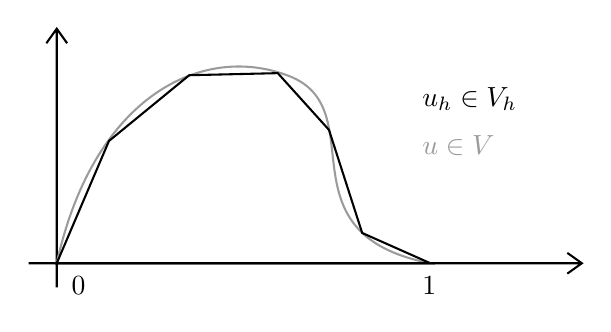
\begin{tikzpicture}[x=0.75pt,y=0.75pt,yscale=-1,xscale=1]
			%uncomment if require: \path (0,159); %set diagram left start at 0, and has height of 159

			%Shape: Axis 2D [id:dp8278071344800375]
			\draw  (156,126.42) -- (422.5,126.42)(169.5,13.42) -- (169.5,138) (415.5,121.42) -- (422.5,126.42) -- (415.5,131.42) (164.5,20.42) -- (169.5,13.42) -- (174.5,20.42)  ;
			%Curve Lines [id:da39265940270590605]
			\draw [color={rgb, 255:red, 155; green, 155; blue, 155 }  ,draw opacity=1 ]   (169.5,126.42) .. controls (187.33,45.5) and (240,20.17) .. (281.33,36.17) .. controls (322.67,52.17) and (276,112.17) .. (349.5,126.42) ;
			%Shape: Polygon [id:\ds4903057462294962]
			\draw   (349.5,126.42) -- (169.5,126.42) -- (194.67,67.5) -- (233.33,35.83) -- (276,34.83) -- (300.67,62.17) -- (316.67,111.83) -- cycle ;

			% Text Node
			\draw (180,137) node    {$0$};
			% Text Node
			\draw (349,137) node    {$1$};
			% Text Node
			\draw (344.17,63.4) node [anchor=north west][inner sep=0.75pt]  [color={rgb, 255:red, 155; green, 155; blue, 155 }  ,opacity=1 ]  {$u\in V$};
			% Text Node
			\draw (344.17,40.4) node [anchor=north west][inner sep=0.75pt]    {$u_{h} \in V_{h}$};


		\end{tikzpicture}
	\end{figure}
	\FloatBarrier
\end{itemize}

Dobbiamo saper stimare l'errore della soluzione approssimata $u_h$ rispetto a quella reale $u$, senza conoscere quest'ultima. Dobbiamo poi trovare un modo per controllare questo errore, cioè renderlo arbitrariamente piccolo.

I passi per costruire $\displaystyle u_{h}$ sono:
\begin{enumerate}
\item Costruiamo lo spazio $V_{h}$. Ricordiamo che $\operatorname{dim}( V_{h}) =N_{h} < +\infty $, e che qualunque spazio di dimensione $\displaystyle N_{h}$ può essere generato da $\displaystyle N_{h}$ vettori indipendenti.
Per indicarlo scriviamo:
\begin{equation*}
V_{h} =\operatorname{span}\{\varphi _{j}(x) ,j=1, \dotsc, N_{h}\}.
\end{equation*}
\item Scriviamo $\displaystyle u_{h}$ come combinazione lineare delle funzioni di base $\displaystyle \varphi _{j}(x)$ secondo i coefficienti $u_j ,j=1,\dotsc ,N_{h}$, ossia
\begin{equation*}
u_{h}(x) =\sum ^{N_{h}}_{j=1} u_{j} \varphi _{j}(x), \quad u_{1} ,u_{2} ,\dotsc ,u_{N_h} \in \mathbb{R} .
\end{equation*}
\item Utilizzando questa espansione riscriviamo \eqref{eq:formulazione-forte}. Trovare $u_{1}, u_{2}, \dotsc, u_{N_h} \in \mathbb{R}$ tali che:
\begin{equation*}
\int\nolimits ^{1}_{0}\sum\limits ^{N_{h}}_{j=1} u_{j} \varphi '_{j}(x) v'_{h}(x) \dx=\int\nolimits ^{1}_{0} f(x) v_{h}(x) \dx,\ \ \ \ \forall v_{h}(x) \in V_{h}.
\end{equation*}
\item Osserviamo che la condizione $\displaystyle \forall v_{h}(x) \in V_{h}$ è equivalente a $\displaystyle \forall \varphi _{i}(x) ,i=1,\dotsc ,N_{h}$. Se l'identità vale per le funzioni di base $\displaystyle \varphi _{i}$ allora vale anche per le funzioni $\displaystyle v_{h}$ dato che si devono poter scrivere come combinazione delle funzioni di base:
\begin{equation*}
v_{h}(x) \ =\ \sum\limits ^{N_{h}}_{i=1} v_{i} \varphi _{i}(x).
\end{equation*}

Si ha dunque il seguente problema. Trovare $u_{1}, u_{2}, \dotsc, u_{N_h} \in \mathbb{R}$ tali che:
\begin{equation*}
\int\nolimits ^{1}_{0}\sum\limits ^{N_{h}}_{j=1} u_{j} \varphi '_{j}(x) \varphi '_{i}(x) \dx=\int\nolimits ^{1}_{0} f(x) \varphi _{i}(x) \dx,\ \ \ \ \forall i=1,\dotsc ,N_{h}.
\end{equation*}
\item Utilizziamo la linearità dell'integrale per affermare che questa espressione è equivalente a un sistema lineare di $N_{h}$ equazioni in $\displaystyle N_{h}$ incognite.
Trovare $u_{1}, u_{2}, \dotsc, u_{N_h} \in \mathbb{R}$ tali che:
\begin{equation*}
\sum\limits ^{N_{h}}_{j=1} u_{j}\int\nolimits ^{1}_{0} \varphi '_{j}(x) \varphi '_{i}(x) \dx=\int\nolimits ^{1}_{0} f(x) \varphi _{i}(x) \dx,\ \ \ \ \forall i=1,\dotsc ,N_{h}.
\end{equation*}

Definiamo:
\begin{gather*}
\mathbf{u} =\begin{bmatrix}
u_{1}\\
u_{2}\\
\vdots \\
u_{N_{h}}
\end{bmatrix} \in \mathbb{R}^{N_{h}} ,\ \ \ \ \mathbf{F} =\begin{bmatrix}
\int ^{1}_{0} f(x) \varphi _{1}(x) \dx\\
\int ^{1}_{0} f(x) \varphi _{2}(x) \dx\\
\vdots \\
\int ^{1}_{0} f(x) \varphi _{N_{h}}(x) \dx
\end{bmatrix} \in \mathbb{R}^{N_{h}} ,\\\\
A=\begin{bmatrix}
\int ^{1}_{0} \varphi '_{1}(x) \varphi '_{1}(x) \dx & \int ^{1}_{0} \varphi '_{1}(x) \varphi '_{2}(x) \dx & \dotsc  & \int ^{1}_{0} \varphi '_{1}(x) \varphi '_{N_{h}}(x) \dx\\
\int ^{1}_{0} \varphi '_{2}(x) \varphi '_{1}(x) \dx & \int ^{1}_{0} \varphi '_{2}(x) \varphi '_{2}(x) \dx & \dotsc  & \int ^{1}_{0} \varphi '_{2}(x) \varphi '_{N_{h}}(x) \dx\\
\vdots  & \vdots  & \ddots  & \vdots \\
\int ^{1}_{0} \varphi '_{N_{h}}(x) \varphi '_{1}(x) \dx & \int ^{1}_{0} \varphi '_{N_{h}}(x) \varphi '_{2}(x) \dx & \dotsc  & \int ^{1}_{0} \varphi '_{N_{h}}(x) \varphi '_{N_{h}}(x) \dx
\end{bmatrix}.
\end{gather*}
Possiamo quindi riassumere il tutto scrivendo
\begin{equation}
	A\mathbf{u} =\mathbf{F}.
	\label{eq:Au-F}
\end{equation}
\end{enumerate}


Di seguito un riassunto del procedimento enunciato, tipico dei problemi di matematica numerica:
\begin{figure}[htpb]
	\centering
	\tikzset{every picture/.style={line width=0.75pt}} %set default line width to 0.75pt

	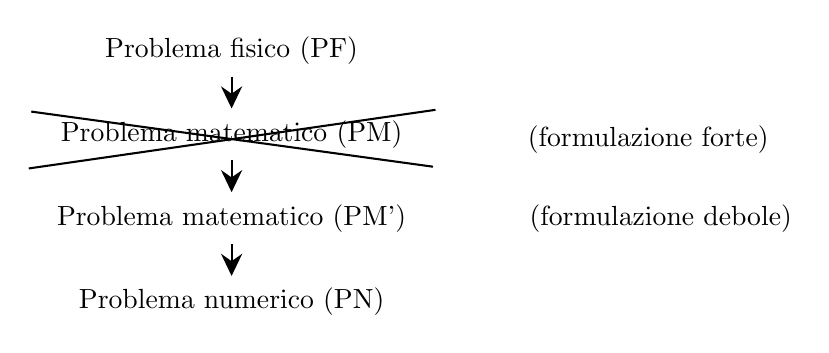
\begin{tikzpicture}[x=0.75pt,y=0.75pt,yscale=-1,xscale=1]
	%uncomment if require: \path (0,176); %set diagram left start at 0, and has height of 176

	%Straight Lines [id:da3784883159291015]
	\draw [line width=0.75]    (113.73,55.32) -- (307.27,81.87) ;
	%Straight Lines [id:da7613061076345762]
	\draw [line width=0.75]    (112.5,82.72) -- (308.5,54.47) ;

	% Text Node
	\draw (210.25,26) node   [align=left] {Problema fisico (PF)};
	% Text Node
	\draw (210.25,66.33) node   [align=left] {Problema matematico (PM)};
	% Text Node
	\draw (210.25,106.66) node   [align=left] {Problema matematico (PM')};
	% Text Node
	\draw (210.25,147) node   [align=left] {Problema numerico (PN)};
	% Text Node
	\draw (411,69) node   [align=left] {(formulazione forte)};
	% Text Node
	\draw (417,107) node   [align=left] {(formulazione debole)};
	% Connection
	\draw    (210.25,38.5) -- (210.25,50.83) ;
	\draw [shift={(210.25,53.83)}, rotate = 270] [fill={rgb, 255:red, 0; green, 0; blue, 0 }  ][line width=0.08]  [draw opacity=0] (10.72,-5.15) -- (0,0) -- (10.72,5.15) -- (7.12,0) -- cycle    ;
	% Connection
	\draw    (210.25,78.83) -- (210.25,91.16) ;
	\draw [shift={(210.25,94.16)}, rotate = 270] [fill={rgb, 255:red, 0; green, 0; blue, 0 }  ][line width=0.08]  [draw opacity=0] (10.72,-5.15) -- (0,0) -- (10.72,5.15) -- (7.12,0) -- cycle    ;
	% Connection
	\draw    (210.25,119.16) -- (210.25,131.5) ;
	\draw [shift={(210.25,134.5)}, rotate = 270] [fill={rgb, 255:red, 0; green, 0; blue, 0 }  ][line width=0.08]  [draw opacity=0] (10.72,-5.15) -- (0,0) -- (10.72,5.15) -- (7.12,0) -- cycle    ;

	\end{tikzpicture}
\end{figure}
\FloatBarrier

Per svolgere questi passaggi è necessario saper:
\begin{itemize}
\item risolvere sistemi lineari,
\item calcolare integrali definiti,
\item approssimare funzioni e dati, e le loro derivate.
\end{itemize}

Se il problema da risolvere dipendesse anche dal tempo, avremmo bisogno di ulteriori strumenti numerici (risoluzione di sistemi di EDO non lineari) che vedremo negli ultimi capitoli.
